\documentclass[DIV=calc,paper=a4,fontsize=11pt,twocolumn]{scrartcl}

\usepackage[german]{babel}
\usepackage[utf8]{inputenc}
\usepackage{fourier}
\usepackage[protrusion=true,expansion=true]{microtype}
\usepackage{amsmath,amsfonts,amsthm}
\usepackage[svgnames]{xcolor}
\usepackage[hang,small,labelfont=bf,up,textfont=it,up]{caption}
\usepackage{booktabs}
\usepackage{fix-cm}
\usepackage{graphicx}
\usepackage{url}

\usepackage{sectsty}
\allsectionsfont{\usefont{OT1}{phv}{b}{n}}

\usepackage{fancyhdr}
\pagestyle{fancy}
\usepackage{lastpage}

% Headers - all currently empty
\lhead{}
\chead{}
\rhead{}

% Footers
\lfoot{}
\cfoot{}
\rfoot{\footnotesize Seite \thepage\ von \pageref{LastPage}}

\renewcommand{\headrulewidth}{0.0pt} % No header rule
\renewcommand{\footrulewidth}{0.0pt} % Thin footer rule

\usepackage{titling}

\newcommand{\HorRule}{\color{DarkGrey}\rule{\linewidth}{2pt}}

\pretitle{\vspace{-50pt}
  \begin{flushleft}
    \HorRule
    \fontsize{30}{30}
    \usefont{OT1}{phv}{b}{n}
    \color{SteelBlue}
    \selectfont}

\title{Patientendaten Sicherheit}

\posttitle{\end{flushleft}\vspace{-10pt}}

\preauthor{\begin{flushleft}\large
    \usefont{OT1}{phv}{b}{n}
    \color{SteelBlue}}

\author{Optinomic GmbH}

\postauthor{\end{flushleft}\vspace{-20pt}}

\predate{\begin{flushleft}
    \usefont{OT1}{phv}{b}{n}
    \color{SteelBlue}}

\date{12. Oktober 2013}

\postdate{\end{flushleft}\vspace{-10pt}\HorRule}

\begin{document}

\maketitle

\thispagestyle{fancy}

{\setlength\parindent{0pt} \textbf{Die Prävalenz von mHealth
    Anwendungen wächst rasant in die europäischen Markt. Die Messung
    des therapierelevanten Patientendaten und die Abgabe von
    therapeutischen Beratung über eigenen Mobilegeräte Patienten
    (Smartphones und Tablets) stellt neue Herausforderungen in der
    Bereich des Datenschutzes. In diesem Papier stellen wir eine
    vorgeschlagene Plan für Verwaltung von Patientendaten in der
    Optinomic Verwaltungsrahmenwerk für Umfrage und kognitiven
    Tests. Dieser Plan soll starken Datenschutz gewährleisten und
    gleichzeitig Flexibilität und Benutzerfreundlichkeit für Patienten
    und Therapeuten unterstützen. Ein kryptographisch sicheren
    Mechanismus verwendet wird um sicherzustellen, dass Patienten
    Umfrageantworten von einem patienteneigenen Mobilgerät gesammelt
    werden können aber nur dann zugeordnet werden, Patienten
    Erkennungsinformationen im Zusammenhang mit einem sicheren Server
    beibehalten hinter einer Klinik-Firewall.}}

\section*{Datenspeicher für mHealth}

Es gibt gute Hinweise, dass Patienten Überwachung der mentalen
Zustände und Abgabe von therapeutischen Materials Patienten außerhalb
einer klinischen Einstellung zu einer verbesserten therapeutischen
Ergebnissen führen kann. Die allgegenwärtige Nutzung von Mobilegeräten
wie Smartphones und Tablets bietet eine klare Gelegenheit, solche
``extraklinischen'' Unterstützung für Patienten bereitzustellen, und
moderne Web-Anwendung-Technologie ermöglicht die Entwicklung von
Rahmenwerken, die Therapeuten helfen können, die Informationen von
ihren Patienten gesammelt zu verwalten und Patientenzustanden zu
überwachen, um in Frühintervention bei eventuellen Problemen
unterzustützen.

Optinomic entwickelt ein Rahmenwerk, das adaptive Überwachung von
Patientenzustanden, Einhaltung der Behandlung und therapeutische
Ergebnisse bieten über Umfragen und einfache kognitive Tests zu
Smartphones, Tablets oder Patienten Schreibtischcomputern
ausgeliefert. Das Optinomic-System integrieren mit bestehenden
Klinikinformationssystems, unterstützt in der Sammlung der gesetzlich
vorgeschriebenen Patienteninformationen (z.B. die Aufnahme Umfragen
erforderlich für die Behandlung von Drogenmissbrauch Erkrankungen) und
verwenden moderne statistische Methoden, um Therapeuten und Forschern
Fortschritt des Patienten effektiver zu modellieren ermöglichen.

Sammlung von Daten mit Mobilgeräten und Internet-Technologien hat
schwerwiegende Folgen für die Einhaltung der datenschutzrechtlichen
Bestimmungen. Patientendaten werden nicht mehr starr in einer Klinik
beschränkt IT-Systeme, wo sie überwacht und gesteuert werden
können. Dies bedeutet, dass eine sorgfältige Analyse notwendig ist, um
sicherzustellen, dass egal welche Methoden verwendet werden, um
Patientendaten zu sammeln, starke Datenschutz gewährleisten.

\section*{Auswirkungen auf die Sicherheit}

Im Rahmen der vorgeschalegenen Anwendungen gibt es zwei Arten von
Informationen, die berücksichtigt werden müssen. Erstens gibt es
\emph{Patienten Erkennungsinformationen}: Namen der Patienten,
einzigartigen innerhalb von Klinikinformationssystems benutzten
Bezeichner, Geschlecht, Geburtsdatum, Krankengeschichte,
E-Mail-Adressen usw. Diese Informationen müssen geschützt werden und
darf zu keiner Einrichtungen außerhalb einer Klinik
Sicherheits-Firewall zugänglich sein.

Die zweite Klasse von Daten umfasst Antworten von Patienten auf
Umfragen und Ergebnisse kognitiven Tests. Diese Daten hat keine
\emph{intrinsische} Vertraulichkeit -- eine Vertraulichkeitpflicht
entsteht nur aus der Möglichkeit einer Zuordnung dieser Daten mit dem
von wem sie stammenen Patienten. Es sollte keine Möglichkeit sein,
Antworten von Patienten auf eine Umfrage zu Patienten
Erkennungsinformationen zu verbinden, \emph{außer} im Rahmen eines
genehmigten System innerhalb der Klinik-Firewall.

Das Kernproblem ist also, dass wir möchten Patienten befähigen,
Optinomic Anwendungen aus den eigenen Mobilgeräten und
Schreibtischcomputern mit dem Browser, dass sie vertraut sind, zu
abrufen, ohne die besonderen Sicherheitsmaßnahmen selbst zu treffen
müssen, während bei Gleichzeitig eine sichere Trennung zwischen
Patienten Erkennungsinformationen und Antworten auf Umfragen
gewährleisten.


\section*{Lösungsvorschlag}

Die Architektur, die wir vorschlagen, ist wie folgt:

\begin{itemize}
  \item{Wir verwenden eine private \emph{Therapieverwaltung-Server},
    die innerhalb der Klinik-Firewall liegt, mitsamt einem öffentlich
    zugänglichen \emph{Umfrage-Server}. Die Therapieverwaltung-Server,
    wobei innerhalb die Klinik-Firewall, wird nach den Sicherheit- und
    Datenschutz-Richtlinien der Klinik verwaltet.}
  \item{Alle Ablaufplanung von Patienten Umfragungen und
    Testaktivitäten wird durch das Therapieverwaltung-Server getan.}
  \item{Die \emph{einzige} Beziehung zwischen einen Patienten und
    seine/ihre Umfrage/Testaktivität ist eine zufällig generierte
    \emph{Umfrage-Ticket}.}
  \item{Es gibt keine Korrelation zwischen Umfrage-Tickets für den
    gleichen Patienten oder zwischen Umfrage-Tickets für die gleiche
    Umfrage oder Test-Modul, und es gibt keine zeitliche Korrelation
    zwischen Tickets damit, korrelationbasierte Angriffe auf
    Ticket-Belegung verhindert werden.}
\end{itemize}

Die Arbeitsweise dieser Architektur lässt sich am besten mit einer
detaillierten Blick auf die primäre Anwendungsfall dargestellt: die
Ablaufplanung, Durchführung und Datensammlung für eine einzelne
Aktivierung von einer Umfrage-Modul für einen einzelnen Patienten.


\section*{Anwendungsfälle}

Der primäre Anwendungsfall, den wir hier präsentieren, ist daß einer
Therapeut einer Patienten-Umfragetätigkeit planen, und die
anschließende Präsentation der Umfrage vor dem Patienten, von der
Datensammlung gefolgt. Dieser Anwendungsfall zeigt die meisten den
einschlägigen Themen in Bezug auf die Sicherheit von den
Patientendaten für unsere Anwendungen auf. Einige weitere
Anwendungsfälle werden unten berücksichtigt.

\subsection*{Primäre Anwendungsfall}

\begin{figure*}
  \begin{center}
    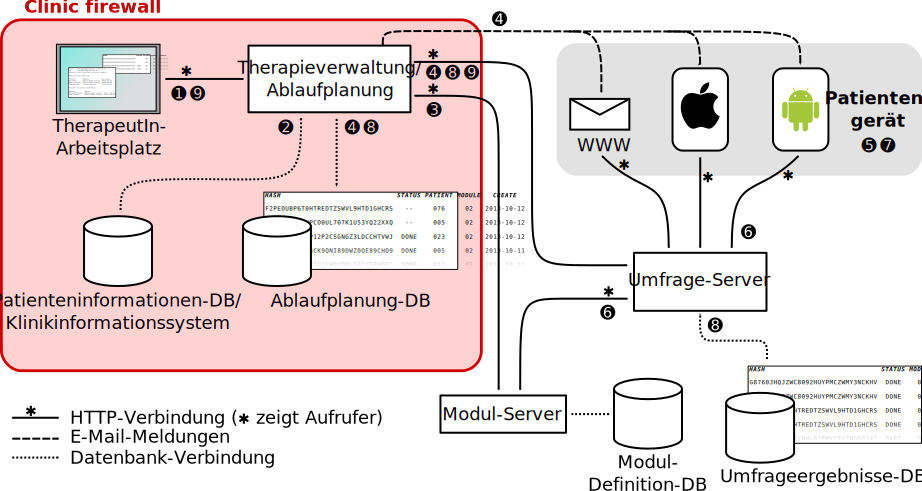
\includegraphics[width=\textwidth]{flow-diagram-de}
  \end{center}
  \caption{Datenflussdiagramm für die primäre
    Umfrage-Ablaufplanung-Anwendungsfall. Siehe Text fur
    Einzelschritterklärung.}
  \label{fig:flow-diagram}
\end{figure*}

Die Benummerung der folgenden Schritte entspricht den nummerierten
Wechselwirkungen in Bild~\ref{fig:flow-diagram}:

\begin{enumerate}
  \item{Der Therapeut interagiert mit dem Optinomic-System von einem
    Arbeitsplatz, der innerhalb der bestehenden IT-Firewall der Klink
    liegt, wo es den Datenschutz-Richtlinien der Klinik zufolge
    verwaltet werden kann. Der Therapeut nutzt einen Web-Browser, um
    mit dem Optinomic Therapieverwaltung-Server zu verbinden, der auch
    innerhalb der Klinik-Firewall liegt. Da sowohl der
    Therapeut-Arbeisplatz als auch der Therapieverwaltung-Server
    innerhalb der Klinik-Firewall liegen, diese Verbindung kann über
    eine normale HTTP-Verbindung gemacht werden. Wenn die
    IT-Richtlinien der Klinik, Therapeuten den Kliniksysteme von
    außerhalb der Klinik-Firewall über VPN oder andere sichere
    Verbindungen abrufen lassen, ist dieser Weg auch eine Option für
    den Anschluss an die Optinomic Server.}
  \item{Der Therapeut kann dann Patientendaten abrufen, indem sie
    entweder eine Verknüpfung zu einem vorhandenen
    Klinikinformationssystem oder eine Optinomic Patientendaten
    Datenbank verwendet. Alle diese Komponenten werden innerhalb der
    Klinik-Firewall enthalten. Sofern die Integrität der
    Klinik-Firewall in irgendeiner Weise nicht verletzt wird, gibt es
    keine Möglichkeit einer Beeinträchtigung der
    Patientendaten. Durchsetzung der Integrität dieser Firewall ist
    über den Umfang des Optinomic Anwendung und ist die Verantwortung
    der Klinik und ihre bestehende Informationssystem-Anbieter.}
  \item{Der Therapeut wählt eine therapeutische Modul (Umfrage oder
    kognitiven Test), um für einen Patienten zu planen, indem sie
    durch Modul-Definitionen auf einem Modul-Server (die \emph{Modul
      Markt}) durchsucht.  Keine Patientdaten wird mit diesen
    Moduldefinitionen assoziiert und der Modul-Server kann daher
    außerhalb der Klinik-Firewall liegen (in vielen Fällen würden wir
    empfehlen, dass Modul-Definitionen aus eine zentrale Optinomic
    Server zugegriffen werden, damit die neuesten Versionen Moduls
    immer erhältlich seien). Der Zugriff auf dem Modul-Server wird von
    der Therapieverwaltung-Server eingeleiteten, anhand von einer
    normalen HTTP-Verbindung.}
  \item{Der entscheidende Arbeitsschritt von der Datenfluß ist die
    Ablaufplanung des Moduls für einen Patienten. Es muss ein
    Zusammenhang zwischen einem persönliche Patienten-Kennnummer und
    eine Instanz der Aktivierung des Moduls gemacht werden. Der
    Patient muss auch darüber informiert, dass das Modul werden zur
    Verfügung, um daran zu arbeiten. Um zu ermöglichen, die Patienten
    mit ihren eigenen Mobilgeräten Umfragen auszufüllen, ohne zu
    Patienten Erkennungsinformationen (Name, einzigartigen
    Patienten-ID, E-Mail-Adresse, usw.) nach Servers außerhalb der
    Klinik-Firewall unströmen lassen, ein statistisches
    \emph{Umfrage-Ticket} erzeugt wird. Diese Umfrage-Ticket ist eine
    32-stellige aus Buchstaben und Ziffern aufgebaute Zeichenfolge,
    die durch die Therapieverwaltung-Server für jedes Aktivierung
    eines Modul erzeugt wird. Die einzige Ort, an dem eine direkte
    Verbindung zwischen diesem zufällige Zeichenfolge und die
    Patienten-ID gemacht wird, ist ein in der Optinomic
    Terminplanung-Datenbank erstellte Eintrag, der innerhalb der
    Klinik-Firewall liegt, und nur durch die Therapieverwaltung-Server
    zugänglich ist. Sobald der Eintrag in der Planung-Datenbank
    erstellt wurde, die Umfrage-Ticket und die Angabe des aktiviert zu
    wordene Moduls werden um das \emph{Umfrage-Server}
    übergeben. Beachten Sie, dass kein Patienten
    Erkennungsinformationen zu dem Umfrage-Server übergeben wird, der
    auf einer Maschine außerhalb der Klinik-Firewall läuft, und kann
    direkt von den Patienten mit den eigenen Mobilegeräten oder
    Schreibtischcomputern abgerufen worden. Die gesamte Verarbeitung
    auf dem Umfrage-Server wird in Bezug auf diesen zufällig
    generierten Umfrage-Tickets getan. Sobald die Umfrage-Server des
    Moduls Aktivierung mitgeteilt worden, die
    Therapieverwaltung-Server sendet eine E-Mail Mitteilung an die
    registrierte E-Mail-Adresse von dem Patienten, um sie zu
    mitteilen, dass ein neues Modul Aktivierung erhältlich
    ist. Beachten Sie wieder, dass E-Mail-Adressen der Patienten wird
    \emph{nicht} an den Umfrage-Server gesendet, obwohl die E-Mail an
    den Patient muss auch die Umfrage-Ticket enhalten, um eine Link
    geben, die der Patient folgen kann, um den Fragebogen
    auszufüllen. Für Kunden, die fühlen, dass ihre
    E-Mail-Infrastruktur bietet keine ausreichende Sicherheit,
    empfehlen wir die Verwendung E-Mail Fremdleistungen, wie Amazon
    AWS, die über ein verschlüsselte HTTPS-Verbindung zugegriffen
    werden kann. Diese Maßnahme würde gegen Angriffe schützen, die aus
    der Klinik E-Mail-Server ausgehenden E-Mails, zu schnüffeln,
    versuchen, um Patienten E-Mails zu erfassen, obwohl es erfordern
    die Klinik, um die Drittanbieter vertrauen.}
  \item{An irgendeinen Zeitpunkt nachher, greift der Patient seine
    E-Mail zu, mit was Mobilgerät oder E-Mail-Client, dass sie
    gewöhnlich verwendet und sie sehen, dass er eine Nachricht von der
    Optinomic Therapieverwalter hat. Diese Nachricht enthält eine auf
    der Umfrage-Ticket vom Therapieverwaltung-Server erzeugt werden
    aufgebaute URL, die auf dem betreffenden Umfrage-Seite führen
    (z.B.
    \url{http://www.optinomic.ch/G8760JHQJZWC8092HUYPMCZWMY3NCKHV}).}
  \item{Wenn der Patient folgt die URL in der E-Mail-Nachricht, die
    Umfrage-Server erzeugt HTML-Seiten und Javascript-Code, um die
    relevanten Umfrage oder kognitiven Test auf dem Mobilgerät oder
    Computer des Patienten zu laufen. Da der Inhalt der Umfrage ist
    nur durch die zufällig generierte Umfrage-Ticket zugegriffen, kann
    diese Verbindung über eine normale HTTP-Verbindung hergestellt
    werden.}
  \item{Der Patient schließt die Umfrage auf seinem Mobilgerät
    ab. Wenn er/sie fertig ist, werden die Ergebnisse der Umfrage zum
    Umfrage-Server übermittelt.}
  \item{Wenn der Server die Ergebnisse einer Umfrage erhält, speichert
    er sie zu einem Umfrageergebnisse Datenbank. Diese Datenbank wird
    vom zufälligen Umfrage-Ticket indiziert, so es keine Mittel gibt,
    dadurch die Ergebnisse der Umfrage mit Patientenidentitäten können
    zugeordnet werden \footnote{Die einzige Ausnahme von dieser
      Aussage ist (natürlich), wenn das Modul direkt über Patienten
      Erkennungsinformationen als Teil einer Umfrage anfragt.}.
    Sobald die Ergebnisse der Umfrage gespeichert werden, sind sie für
    die Therapieverwaltung-Server erhältlich, der die Umfrage-Server
    regelmäßig pollt (alle etwa paar Minuten), um die Umfrage-Tickets
    für alle vor kurzem abgeschlossenen Umfragen zu verlangen. (Der
    Therapieverwaltung-Server bestimmt diese Informationen durch
    Polling, statt zu direkt vom Umfrage-Server mitgeteilt wird, um
    die Notwendigkeit der Umfrage-Server eine eingehende Verbindung
    über den Klinik-Firewall etablieren zu vermeiden.)  Wenn die
    Therapieverwaltung-Server bestimmt, dass eine Untersuchung
    abgeschlossen ist, aktualisiert es die Ablaufplanung-Datenbank, um
    anzuzeigen, dass der Patient den zugeordneten Aktivität
    abgeschlossen hat (an dieser Stelle, die Verwaltung-Server konnte
    auch Warnungen an den Therapeuten schicken, Anschlussaktivitäten
    für den Patienten auslösen, usw.).}
  \item{Zu irgendeineim späteren Zeitpunkt, anschließt der Therapeut
    wieder an die Therapieverwaltung-Server, um die Ergebnisse der
    Umfrage zu betrachten. Die Therapieverwaltung-Server kann diese
    Ergebnisse vom Umfrage-Server mit einem normalen HTTP-Verbindung
    abrufen. Da der Therapieverwaltung-Server kann sowohl die
    Ergebnisse der Umfrage Datenbank (über die Umfrage-Server) als
    auch die Ablaufplanung-Datenbank Zugang erhalten, kann er die
    Umfrageergebnisse mit Patientenidentitäten in Verbundung über den
    Link zwischen den zufälligen Umfrage-Tickets und in der
    Ablaufplanung-Datenbank gespeicherten Patientenidentitäten
    bringen.}
\end{enumerate}


\subsection*{Andere Anwendungsfälle}

Es gibt eine Auswahl von anderen Anwendungsfällen, die in Bezug auf
die Fragen der Datensicherheit entsprechend sind. Hier erwähnen wir
drei, um anzuzeigen, wie typische Verwendungen des Optinomic Systems
unwahrscheinlich können, eine Gefährdung der Vertraulichkeit der
Patientendaten zur Folge haben.

\paragraph{Unterbrechung und Wiederaufnahme der Umfragen}

Bei größeren Umfragen, kann es wünschenswert sein, dass die Patienten
in der Lage sind, die Fertigstellung der Umfrage unterzubrechen und
später fortzusetzen. Es gibt hier zwei mögliche Ansätze: wenn wir
zulassen, Aktivitäten nur auf dem gleichen Gerät anzugehalten und
fortzugesetzt werden, dann können Zwischenergebnisse der Umfrage
einfach in einem Browser-Cookie für den späteren Zugriff gespeichert
werden. Auf der anderen Seite, wenn ein Patient teilweise eine Umfrage
auf einem Gerät (einem Schreibtischcomputer, vielleicht) ausfüllen
will, dann die Umfrage auf einem anderen Gerät (einem Smartphone,
z.B.) beenden, können dann teilweise Ergebnisse der Umfrage, auf der
Umfrage-Server abgespeichert werden. Keiner dieser Ansätze riskiert
Gefährdung das Bindeglied zwischen Patientenidentität und
Umfrageergebnisse.

\paragraph{Patientenüberwachung}

Die aus den Umfrage-Server nach dem Therapieverwaltung-Server
gesendete Nachrichten über den Abschluss von Umfragen ermöglichen
sofortigen Benachrichtigung der Therapeuten, wenn Patienten bestimmte
Tätigkeiten vervollständigen. Da alle Planung und Umfrage
Abschlussinformationen in der Ablaufplanung-Datenbank sich finden,
kann der Therapieverwaltung-Server einfach Berichte von der Aktivität
des Patienten für Therapeuten Überwachung erzeugen, und kann auch den
Therapeut über beunruhigenden Muster von Nichteinhaltung der Patienten
warnen. Die gesamte Datenverarbeitung, die Vereinigung zwischen
Umfrageergebnisse und Patientenidentitäten erfordert, tritt
ausschließlich innerhalb der Klinik-Firewall auf, damit gibt es keine
Gefahr der Verletzung von Patienten Vertraulichkeit.

\paragraph{Zeitliche Veränderung}

Einer der wichtigsten Vorteile des extraklinischen Patienten
Überwachung durch Optinomic vorgeschlagen ist, dass es ermöglicht,
laufende Überwachung von Fortschritt und emotionale Zustände der
Patienten. Automatisierte Ablaufplanung der Sammlung von
Patientendaten über leichte tägliche ``Mini-Umfragen'' ermöglicht die
Ansammlung von langen Zeitreihen von Patientendaten.  Zusammen mit
einfachen Daten-Visualisierung, ermöglicht dies, der Therapeuten
therapeutischen Fortschritt für die Patienten in einer sehr direkten
Art zu demonstrieren: z.B., ``Im letzten Monat, Ihre tägliche
selbsteingeschätzte Stimmung-Punktzahle waren durchweg höher als in
jedem der vorangegangenen drei Monate''. Auch für solche Datenanalyse
werden alle Daten, deren Verarbeitung die Verbindung der
Umfrageergebnisse mit Patientenidentitäten erfordern, tritt
ausschließlich innerhalb der Klinik-Firewall auf, damit es keine
Gefahr der Verletzung der ärztlichen Schweigepflicht gibt.


\section*{Schlussfolgerungen}

Die vorgeschlagene Aufteilung zwischen der Lagerung von Patienten
Erkennungsinformationen und Umfrage/Testergebnisse anhand von zufällig
generierten Umfrage-Tickets, die Verbindung zwischen den beiden Arten
von Daten bereitzustellen, bietet starken Schutz gegen Verletzungen in
Vertraulichkeit der Patientendaten (vorausgesetzt natürlich, dass die
zugrunde liegenden IT-Sicherheitsinfrastruktur selbst nicht
beeinträchtigt ist). Innerhalb des Optinomic Rahmenwerks, gibt es kein
Durchfluss von Patienten Erkennungsdaten aus der Klinik-Firewall,
außer die kleine Möglichkeit der Zuordnung Patient-E-Mail-Adressen und
Umfrage-Tickets, wenn die Sicherheit der Klinik E-Mail-System verletzt
ist.  Abgesehen von dieser E-Mail-Schnüffeln-Angriffsmethode, gibt es
keine Möglichkeit einer Verbindung zwischen Patient Umfrageergebnisse
und Patientenidentitäten außerhalb der Firewall zu machen, weil die
einzige Patientenidentitäten und Umfrage-Tickets zuordnende
Information im Optinomic Ablaufplanung-Datenbank gespeichert ist, die
innerhalb der Klinik-Firewall befindet.

\end{document}
